{\scriptsize%
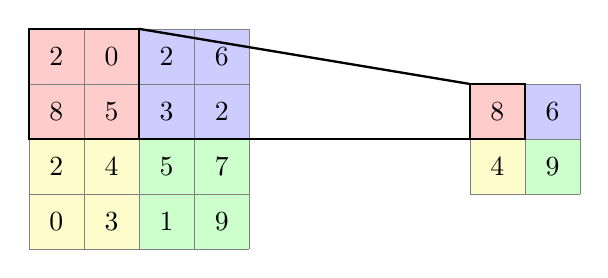
\begin{tikzpicture}[scale=0.7]
    \fill[yellow!20] (0,0) rectangle (2,2);
    \fill[red!20] (0,2) rectangle (2,4);
    \fill[green!20] (2,0) rectangle (4,2);
    \fill[blue!20] (2,2) rectangle (4,4);

    \draw[gray,very thin] (0,0) grid (4,4);

    \node at (0.5,0.5) {0};
    \node at (1.5,0.5) {3};
    \node at (0.5,1.5) {2};
    \node at (1.5,1.5) {4};

    \node at (2.5,0.5) {1};
    \node at (3.5,0.5) {9};
    \node at (2.5,1.5) {5};
    \node at (3.5,1.5) {7};

    \node at (0.5,2.5) {8};
    \node at (1.5,2.5) {5};
    \node at (0.5,3.5) {2};
    \node at (1.5,3.5) {0};

    \node at (2.5,2.5) {3};
    \node at (3.5,2.5) {2};
    \node at (2.5,3.5) {2};
    \node at (3.5,3.5) {6};

    \fill[yellow!20] (8,1) rectangle (9,2);
    \fill[red!20] (8,2) rectangle (9,3);
    \fill[green!20] (9,1) rectangle (10,2);
    \fill[blue!20] (9,2) rectangle (10,3);

    \draw[gray,very thin] (8,1) grid (10,3);

    \node at (8.5,1.5) {4};
    \node at (9.5,1.5) {9};
    \node at (8.5,2.5) {8};
    \node at (9.5,2.5) {6};

    \draw[draw=black, line width=0.3mm] (0,2) rectangle (2,4);
    \draw[draw=black, line width=0.3mm] (8,3) rectangle (9,2);

    \draw[-, line width=0.3mm] (2,4) -- (8,3);
    \draw[-, line width=0.3mm] (2,2) -- (8,2);

\end{tikzpicture}
}
